% report_short.tex -- short synthesis of report.tex (Part I, simulation)
% Build: cd docs/latex && pdflatex report_short && pdflatex report_short
\documentclass[11pt,a4paper]{article}
\usepackage[T1]{fontenc}
\usepackage[utf8]{inputenc}
\usepackage{lmodern}
\usepackage[margin=2.0cm]{geometry}
\usepackage{amsmath}
\usepackage{graphicx}
\usepackage{booktabs}
\usepackage{tabularx}
\usepackage{longtable}
\usepackage{xcolor}
\usepackage{caption}
\usepackage{float}
\usepackage{microtype}
\usepackage{xspace}
\usepackage[colorlinks=true,linkcolor=blue!50!black,urlcolor=blue!50!black]{hyperref}

\captionsetup{font=small,labelfont=bf,margin=0.3cm}
\setlength{\parskip}{0.4em}
\setlength{\parindent}{0pt}
\setlength{\emergencystretch}{3em}
\renewcommand{\arraystretch}{1.15}
\newcolumntype{L}{>{\raggedright\arraybackslash}X}

\newcommand{\pip}{\ensuremath{\pi^{+}}\xspace}
\newcommand{\pim}{\ensuremath{\pi^{-}}\xspace}
\newcommand{\piz}{\ensuremath{\pi^{0}}\xspace}
\newcommand{\ee}{\ensuremath{e^{+}e^{-}}\xspace}
\newcommand{\pipi}{\ensuremath{\pi^{+}\pi^{-}}\xspace}
\newcommand{\ppee}{\ensuremath{\pi^{+}\pi^{-}e^{+}e^{-}}\xspace}
\newcommand{\Mfour}{\ensuremath{M(\pi^{+}\pi^{-}e^{+}e^{-})}\xspace}
\newcommand{\Mee}{\ensuremath{M(e^{+}e^{-})}\xspace}
\newcommand{\Mpipi}{\ensuremath{M(\pi^{+}\pi^{-})}\xspace}
\newcommand{\nbinv}{\ensuremath{\mathrm{nb}^{-1}}\xspace}
\newcommand{\GeVcc}{\ensuremath{\mathrm{GeV}/c^{2}}\xspace}
\newcommand{\MeVcc}{\ensuremath{\mathrm{MeV}/c^{2}}\xspace}
\newcommand{\Lsim}{\ensuremath{L_{\mathrm{sim}}}\xspace}
\newcommand{\Ldata}{\ensuremath{L_{\mathrm{data}}}\xspace}
\newcommand{\code}[1]{\texttt{\detokenize{#1}}}
\newcommand{\notebox}[1]{\par\noindent\colorbox{orange!10}{\parbox{\dimexpr\linewidth-2\fboxsep\relax}{#1}}\par}

\title{\Large $p + p \to \pi^{+}\pi^{-}e^{+}e^{-}$ Analysis Report\\[0.3em]
       \normalsize Short summary of Part I: simulation}
\author{W.~Przygoda}
\date{13 November 2026}

\begin{document}
\maketitle

\notebox{Summary of the full report \code{report.pdf} (45 pages), where every number is derived and
documented. Simulation only: no measured data and no combinatorial background (CB). Expected numbers
of rows in data use $\Ldata = 6080.5\,\nbinv$, which is \textbf{not yet confirmed}.}

{\footnotesize
\setlength{\tabcolsep}{4pt}
\renewcommand{\arraystretch}{1.08}
\begin{longtable}{@{}>{\raggedright\arraybackslash}p{3.3cm} >{\raggedright\arraybackslash}p{\dimexpr\textwidth-3.3cm-2\tabcolsep\relax}@{}}
\caption{\textbf{Notation} used in this summary, in the order of appearance. The full report defines
every item in detail (its ``Notation and abbreviations'' table points to the sections).}
\label{tab:nota}\\
\toprule
\multicolumn{2}{@{}l}{\textbf{Samples and normalisation}} \\
SMASH, PLUTO, HGeant & event generator; decay generator used by the converter; GEANT3-based detector simulation of HADES \\
DST, PAT, FAT & reconstructed data; PostDST Analysis Tool (hypotheses, PID, ranking); Final Analysis Tool (selection, kinematics) \\
$T$, $b_{\max}$, $N$ & beam kinetic energy; largest impact parameter of SMASH; number of simulated events per set \\
\Lsim, \Ldata & integrated luminosity of one simulated set (221.05\,\nbinv); of the data (6080.5\,\nbinv, not confirmed) \\
std, lep, $\eta$ set & the three simulation sets (natural decays; dilepton decays forced; $\eta$ decays forced) \\
row & one combination \pip\pim$e^+e^-$ of reconstructed tracks; an event can give several rows \\
isBest & PAT ranking of the combinations of an event (1 = best, 0 = others); ``all combinations'' = isBest $\ge 0$ \\
PT3 & the physics trigger used for this analysis (bit 8192 of the trigger word) \\
``pre'' & base selection: isBest $\ge0$, vertex $z>-500$\,mm, PT3, vertex $z>-160$\,mm (target), corrected momenta \\
\midrule
\multicolumn{2}{@{}l}{\textbf{Cross sections and counts}} \\
$\sigma_{\mathrm{prod}}$ & production cross section of a particle in SMASH (mean number per collision $\times\,\pi b_{\max}^2$) \\
BR & branching ratio (PDG values unless stated) \\
$\varepsilon$ & acceptance $\times$ efficiency: reconstructed rows after ``pre'' per generated decay \\
$\sigma_{\mathrm{vis}}$ & visible cross section of rows after ``pre'', $\sigma_{\mathrm{prod}}\times\mathrm{BR}\times\varepsilon$; rows at \Ldata $=\sigma_{\mathrm{vis}}\Ldata$ \\
bump, peak & $\eta\to\pipi\piz$ seen below $m_\eta$ (photon lost); $\eta$ seen at $m_\eta$ ($\eta\to\ppee$ or $\eta\to\pipi\gamma$ with conversion) \\
conversion & a photon converted into an \ee pair in the detector material \\
X17 & hypothetical boson of 17\,\MeVcc decaying into \ee; $\mathrm{BR} = \mathrm{BR}(\eta\to\pipi X17)\,\mathrm{BR}(X17\to\ee)$ \\
physical background & rows with a true \ee pair from one source (\piz/$\eta$ Dalitz decay, conversion, $\rho,\omega,\phi$) and any pions \\
multi-pion & physical background from \piz Dalitz and conversion pairs with pions (no $\eta$) \\
fake lepton; two sources & a lepton slot holds a non-lepton or a ghost track; the two leptons come from different decays \\
CB & combinatorial background of the data (absent in simulation) \\
\midrule
\multicolumn{2}{@{}l}{\textbf{Corrections}} \\
\code{geninfo} & generator code of a GEANT track (decay channel), stored by PAT as a 32-bit float \\
rules v2 & weight rules with the exact HGeant branching ratios (from the HGeant card \code{ETA}) \\
QED (Kroll--Wada), form factor & physical distribution of \Mee in a decay through a virtual photon; its hadronic modification \\
OA & opening angle between $e^+$ and $e^-$ (lab) \\
\midrule
\multicolumn{2}{@{}l}{\textbf{Kinematic variables and cuts}} \\
\Mfour, \Mee, \Mpipi & invariant mass of \ppee, of the \ee pair, of the \pipi pair \\
$\mathrm{MM}_4$ & missing mass of \ppee: mass of (beam + target $-$ \pip\pim$e^+e^-$) four-momenta; for $pp\to pp\eta$ it is $M(pp)$ \\
$\alpha_{\mathrm{lab}}$ & angle between the momenta of the \pipi and the \ee systems (lab) \\
$\alpha_\eta$ & angle between \pipi and \ee in the rest frame of a hypothetical $\eta$ with the measured \ppee momentum and mass $m_\eta$ \\
$\Delta z_\pi$ & largest distance in $z$ between a pion track (closest approach to the beam axis) and the event vertex \\
pions in the vertex fit & both pion tracks were used in the fit of the event vertex (PAT flag \code{isUsedVertex}) \\
peak / bump window & $0.5333\le\Mfour<0.5587$ / $0.4576\le\Mfour<0.5255$\,\GeVcc \\
$S$, $B$ & expected signal rows and other (physical-background) rows in a window at \Ldata \\
purity, efficiency & $S/(S+B)$; fraction of the signal of ``pre'' kept by the cuts \\
$F$ & figure of merit $S/\sqrt{S+B}$ \\
\midrule
\multicolumn{2}{@{}l}{\textbf{Test of the extraction}} \\
half A / B & the simulated events split in two (even / odd event-group number): templates from A, pseudo-data from B \\
toy & one pseudo-data set drawn from half B (Poisson bootstrap) \\
bias; pull & mean (extracted $-$ true) over the toys; (extracted $-$ true)/quoted error \\
coverage & fraction of toys whose quoted error contains the truth (0.68 expected) \\
UL & expected 90\,\% CL upper limit on the X17 branching ratio \\
\bottomrule
\end{longtable}
}

%======================================================================
\section{Samples and normalisation}
%======================================================================
\begin{itemize}
\item One SMASH run, p+p at $T = 4.5$\,GeV, $10^{10}$ events, impact parameter uniform in the area up to
      $b_{\max} = 1.2$\,fm (checked in the SMASH configuration and output). Each event stands for
      $\pi b_{\max}^2/N$, so every set has $\Lsim = 221.05\,\nbinv$.
\item Three sets of the \emph{same} events (event by event identical generator content; HGeant rotates
      each event by a random azimuth): \textbf{standard} (all decays natural), \textbf{lepton} (every
      \piz, $\eta$, $\rho^0$, $\omega$, $\phi$ forced into a dilepton channel), \textbf{$\eta$} (every $\eta$
      forced: 50\,\% $\eta\to\ppee$, 50\,\% $\eta\to\pipi X17$).
\item Chain: HGeant, DST (feb22, gen4), PAT (PostDST Analysis Tool, simulation PID cuts) and FAT (Final
      Analysis Tool). Base selection ``pre'': all combinations ($\mathrm{isBest}\ge0$), reconstructed
      vertex $z>-500$\,mm, PT3 trigger, target region $z>-160$\,mm, momenta corrected for energy loss.
\end{itemize}

%======================================================================
\section{Channels, cross sections and expected counts}
%======================================================================
All cross sections here are \emph{visible} cross sections of reconstructed rows after ``pre'':
$\sigma_{\mathrm{vis}} = \sigma_{\mathrm{prod}}\times\mathrm{BR}\times\varepsilon$, with the production from the
SMASH model, the branching ratios from PDG and the acceptance times efficiency $\varepsilon$ from the HADES
simulation.

\begin{table}[H]
\centering
\caption{Signal channels (notation: Table~\ref{tab:nota}). $\sigma_{\mathrm{prod}}(\eta) = 1.0665\pm0.0016$\,mb (SMASH: 0.0236 $\eta$ per
collision). $\varepsilon$: reconstructed rows per generated decay after ``pre''. $\sigma_{\mathrm{vis}}$ with
the physical decay kinematics (QED and form factors for the direct decay, measured Dalitz plot of
$\eta\to\pipi\piz$, pion form factor for $\eta\to\pipi\gamma$). Rows: expected at $\Ldata$, all \Mfour.
X17 for an illustrative $\mathrm{BR}=10^{-5}$.}
\label{tab:ch}
\small
\setlength{\tabcolsep}{4pt}
\begin{tabular}{@{}l l l r r r@{}}
\toprule
 & Process & BR (PDG) & $\varepsilon$ & $\sigma_{\mathrm{vis}}$ [nb] & rows at \Ldata \\
\midrule
bump      & $\eta\to\pipi\piz$, $\piz\to\ee\gamma$                 & $0.2292\times0.01174$ & $2.5\times10^{-3}$ & $7.05\pm0.20$ & 42\,900 \\
bump      & $\eta\to\pipi\piz$, one \piz photon converts            & $0.2292\times0.98823$ & $2.1\times10^{-5}$ & $5.19\pm0.17$ & 31\,600 \\
peak      & $\eta\to\pipi\gamma$, the photon converts              & 0.0422 & $2.8\times10^{-5}$ & $1.24\pm0.07$ & 7\,500 \\
peak      & $\eta\to\ppee$ (direct)                                 & $2.68\times10^{-4}$ & $5.0\times10^{-3}$ & $1.417\pm0.003$ & 8\,600 \\
X17       & $\eta\to\pipi X17$, $X17\to\ee$                         & $10^{-5}$ (hyp.) & $6.7\times10^{-3}$ & 0.0712 & 430 \\
\midrule
\multicolumn{4}{@{}l}{physical background (true \ee pair from one source, any pions)} & 686 & $4.17\times10^{6}$ \\
\multicolumn{4}{@{}l}{\quad of which multi-pion (\piz Dalitz and conversion pairs): 94\,\%} & & \\
\multicolumn{4}{@{}l}{fake lepton / leptons from two sources (shown, not added)} & 125 / 12.5 & \\
\bottomrule
\end{tabular}
\end{table}

The simulated spectrum after ``pre'' (Fig.~\ref{fig:spec}) is dominated by the multi-pion background;
the $\eta$ structures sit on top of it. Conversions are 42\,\% of the simulated bump and almost half of
the peak.

\begin{figure}[H]
\centering
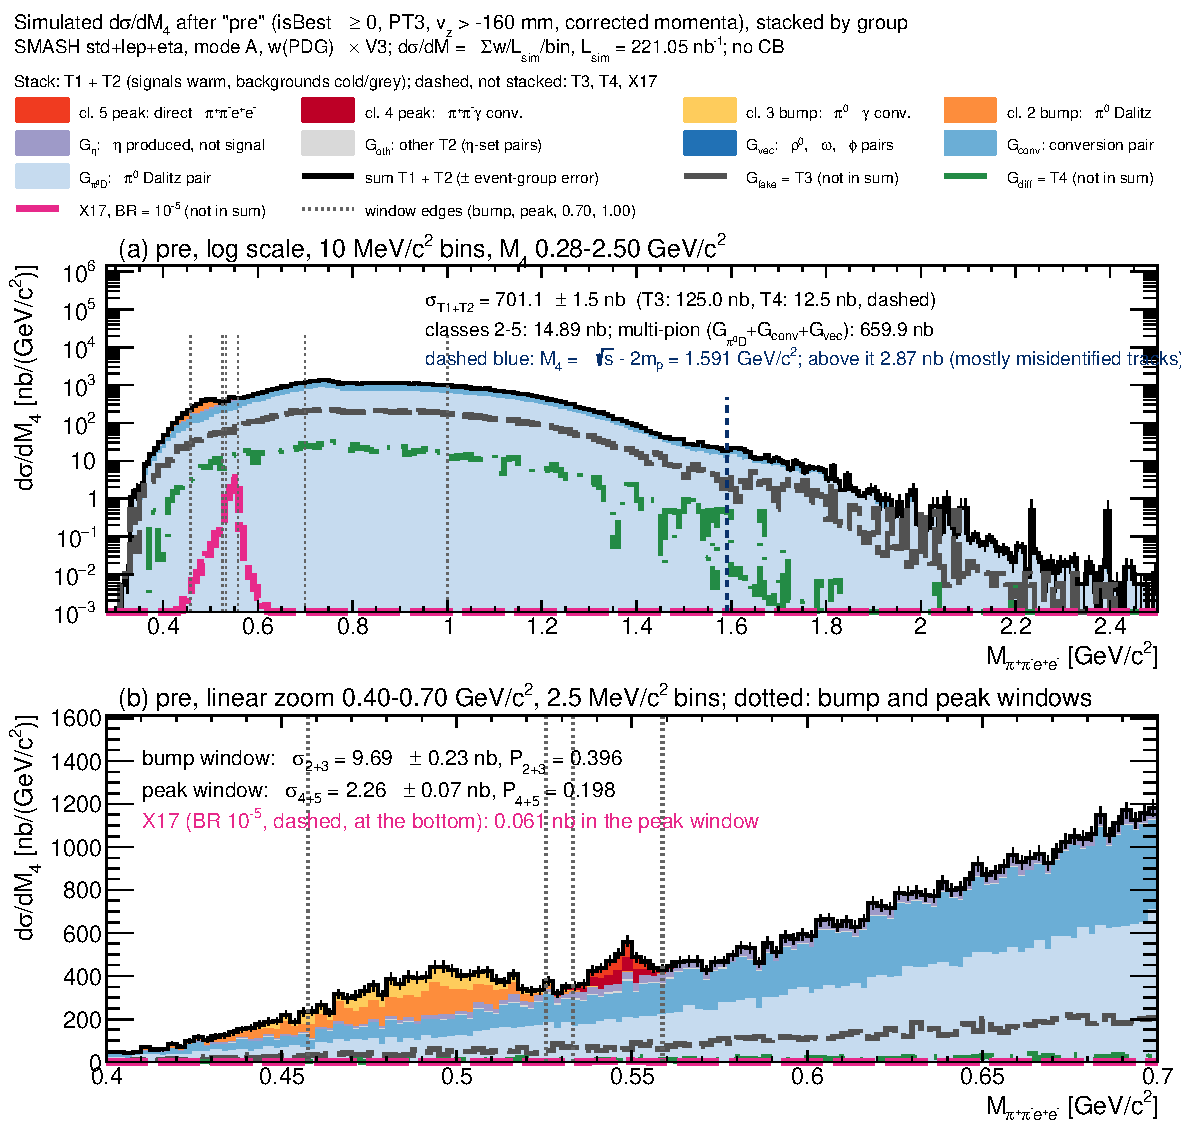
\includegraphics[width=\textwidth]{figs/s5_spec_full_pre.pdf}
\caption{Simulated $d\sigma/d\Mfour$ after ``pre'', stacked by component: signal classes (warm colours)
and background groups (cold colours). Dashed, not stacked: fake leptons, leptons from two sources and X17
at $\mathrm{BR}=10^{-5}$.}
\label{fig:spec}
\end{figure}

%======================================================================
\section{What was corrected}
%======================================================================
\begin{enumerate}
\item \textbf{Generator codes stored as 32-bit floats.} Codes above $2^{24}$ are rounded in the PAT ntuples
      (e.g.\ $\eta\to\ppee$: 1\,702\,030\,809 is stored as 1\,702\,030\,848). All values were mapped back
      unambiguously; a cut \code{TTree::Draw("x==1702030809")} selects nothing.
\item \textbf{Weights of the lepton set.} Same decay = equal (\code{geninfo}, \code{geninfo2}), not the triple
      of the producers' note (that rule weights a Dalitz lepton paired with its own conversion lepton
      83 times too low); the weight of a row is the product over the distinct forced decays of all four
      tracks (leptons also occur in pion slots); the converter's second-decay weight needs a factor 0.0985.
\item \textbf{Ownership between sets.} Every row type is taken from one set only; the sets agree where they
      overlap (non-forced rows of the $\eta$ set against the standard set: $1.0056\pm0.0036$).
\item \textbf{HGeant $\eta$ decay table.} The HGeant input of the production sets
      $\mathrm{BR}(\eta\to\ee\gamma) = 6.0\,\%$ instead of 0.60\,\% (card \code{ETA 37.30 30.20 21.00 4.75 6.0 7.1e-2}).
      Weights now use the exact card values (rules v2): bump $-1.7\,\%$, conversion peak $+3.9\,\%$.
\item \textbf{The $\eta\to\ppee$ generator.} The channel is defined without a dilepton (virtual photon), so
      its \Mee is not QED (27\,\% of the pairs within 0.5\,\MeVcc of threshold, 4.7\,\% above 20\,\MeVcc
      against 28\,\% in QED). Rows are reweighted to Kroll--Wada with form factors; the cut OA$>2^\circ$
      then keeps 0.70 of the simulated peak (0.59 before; data 0.78). The PLUTO plugin \code{eta_physics}
      stays off on purpose; the producers should define the channel as \code{eta:dilepton[e+,e-],pi+,pi-}.
\item \textbf{Bookkeeping.} Simulation PT3 rows have \code{trigbit} 12288 (bit test needed); the merged
      files contain several key cycles (use the highest); rows are grouped into events by adjacency;
      weighted sums in double precision (\code{TH1F} lost 3.4\,\%).
\end{enumerate}

%======================================================================
\section{Final selection}
%======================================================================
The cuts were optimised on simulation truth with $F = S/\sqrt{S+B}$, an exhaustive scan of nine cut
variables, a rule fixed in advance (fewest cuts within 5\,\% of the best $F$ on the full sample and on
both halves) and a split-half check of the optimisation bias (below 1\,\% for the chosen cuts).

\begin{table}[H]
\centering
\caption{Frozen selections (all in addition to ``pre''; notation: Table~\ref{tab:nota}). $S$, $B$: signal and background rows in the
window at \Ldata. $\Delta z_\pi$: largest distance in $z$ of the two pion tracks from the event vertex.}
\label{tab:sel}
\small
\setlength{\tabcolsep}{4pt}
\begin{tabularx}{\textwidth}{@{}>{\raggedright\arraybackslash}p{4.3cm} L r r c c@{}}
\toprule
Target & Cuts & $S$ & $B$ & purity & efficiency \\
\midrule
peak (direct + conversion), $0.5333\le\Mfour<0.5587$ & $\Delta z_\pi<40$\,mm, $\mathrm{MM}_4<2.85$\,\GeVcc & 12\,800 & 41\,800 & 0.23 & 0.93 \\
direct decay only, same window & $\Delta z_\pi<40$\,mm & 7\,100 & 52\,500 & 0.12 & 0.96 \\
bump, $0.4576\le\Mfour<0.5255$ & none & 58\,900 & 89\,800 & 0.40 & 1 \\
X17, peak window & $15.5\le\Mee<24.5$\,\MeVcc, both pions in the vertex fit & 213 at $10^{-5}$ & 5\,340 & & \\
\bottomrule
\end{tabularx}
\end{table}

\begin{itemize}
\item The optimum is flat: many selections are within a few per cent of the best $F$. The gain of the frozen
      peak cuts over ``pre'' is 5\,\% in $F$.
\item The usual $\eta$ cuts (OA$>2^\circ$, $\alpha_{\mathrm{lab}}$, \Mpipi, $\alpha_\eta$) remove background
      \emph{outside} the windows but do not improve them; OA$>2^\circ$ costs 19\,\% of the direct decay. In data
      they may still pay off against the CB, which the simulation does not contain: to be tested on data.
\item $\Delta z_\pi$ is not yet available in the data compact rows; the data-ready equivalent on the plateau is
      ``both pions in the vertex fit''.
\item X17: expected 90\,\% CL limit $1.9\times10^{-5}$ (at \Ldata), set by the simulation statistics of the
      background; $5.7\times10^{-6}$ if the background were known exactly.
\end{itemize}

%======================================================================
\section{Signal extraction compared with the truth}
%======================================================================
The methods planned for data were applied blind to pseudo-data: half of the simulated events gave the
templates, the other half 200 Poisson-bootstrap toys (and 1500 parametric toys for X17); the true content
was revealed only after the procedure was frozen. Fig.~\ref{fig:toy} shows one toy with the fits,
Table~\ref{tab:blind} and Fig.~\ref{fig:bias} the result.

\begin{figure}[H]
\centering
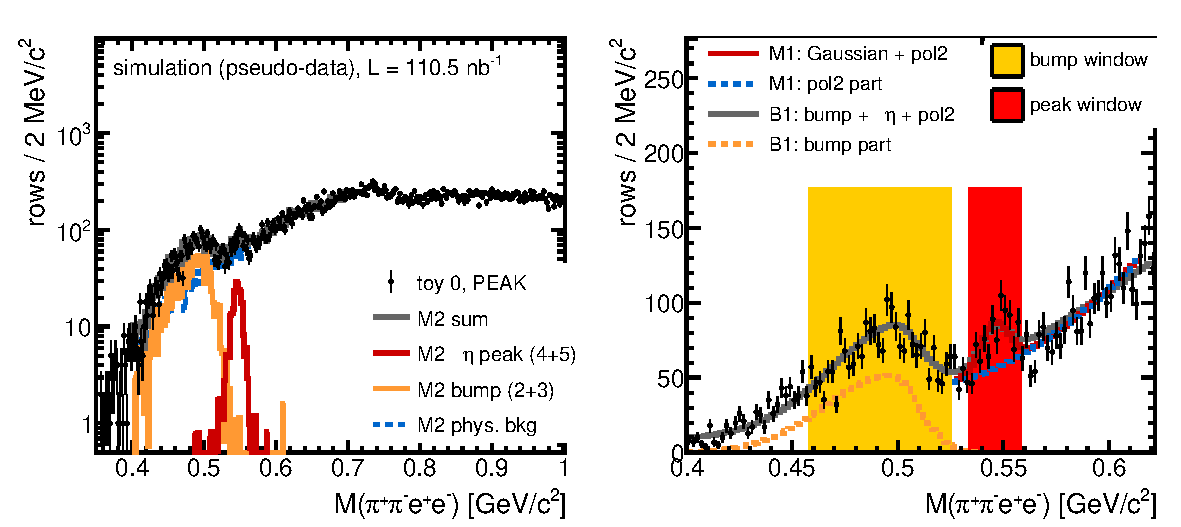
\includegraphics[width=\textwidth]{figs/s5_blind_ana_toy0_PEAK.pdf}
\caption{One pseudo-data toy (110.5\,\nbinv, peak selection). Left: \Mfour with the components of the
template fit. Right: zoom with the Gaussian + polynomial fit of the peak and the parametric fit of the
bump, with the bump and peak windows.}
\label{fig:toy}
\end{figure}

\begin{table}[H]
\centering
\caption{Extracted yield against the truth, mean over 200 toys (notation: Table~\ref{tab:nota}). The common uncertainty of the simulation
templates ($\pm$11--15\,\% peak, $\pm$4.5--5\,\% bump) is shared by all methods. Coverage: fraction of toys
within the quoted error (nominal 0.68).}
\label{tab:blind}
\small
\begin{tabularx}{\textwidth}{@{}>{\raggedright\arraybackslash}p{2.3cm} >{\raggedright\arraybackslash}p{5.0cm} r c L@{}}
\toprule
Yield & Method & bias & coverage & verdict \\
\midrule
peak   & template fit                         & $+1.4\,\%$  & 0.77 & good \\
       & Gaussian + polynomial, calibrated    & $+3.1\,\%$  & 0.72 & good \\
       & linear side bands                    & $-21\,\%$   & 0.53 & loses signal: do not use \\
bump   & side band with simulated shape       & $+3.9\,\%$  & 0.66 & good \\
       & edge step                            & $+1.3\,\%$  & 0.76 & unbiased, 16\,\% error \\
       & template fit / parametric fit        & $+7.7$ / $+5.4\,\%$ & 0.31 / 0.66 & somewhat high \\
direct decay alone & template fit, conversion constrained & $+21\,\%$ & 0.62 & limited by the conversion template \\
\bottomrule
\end{tabularx}
\end{table}

\begin{figure}[H]
\centering
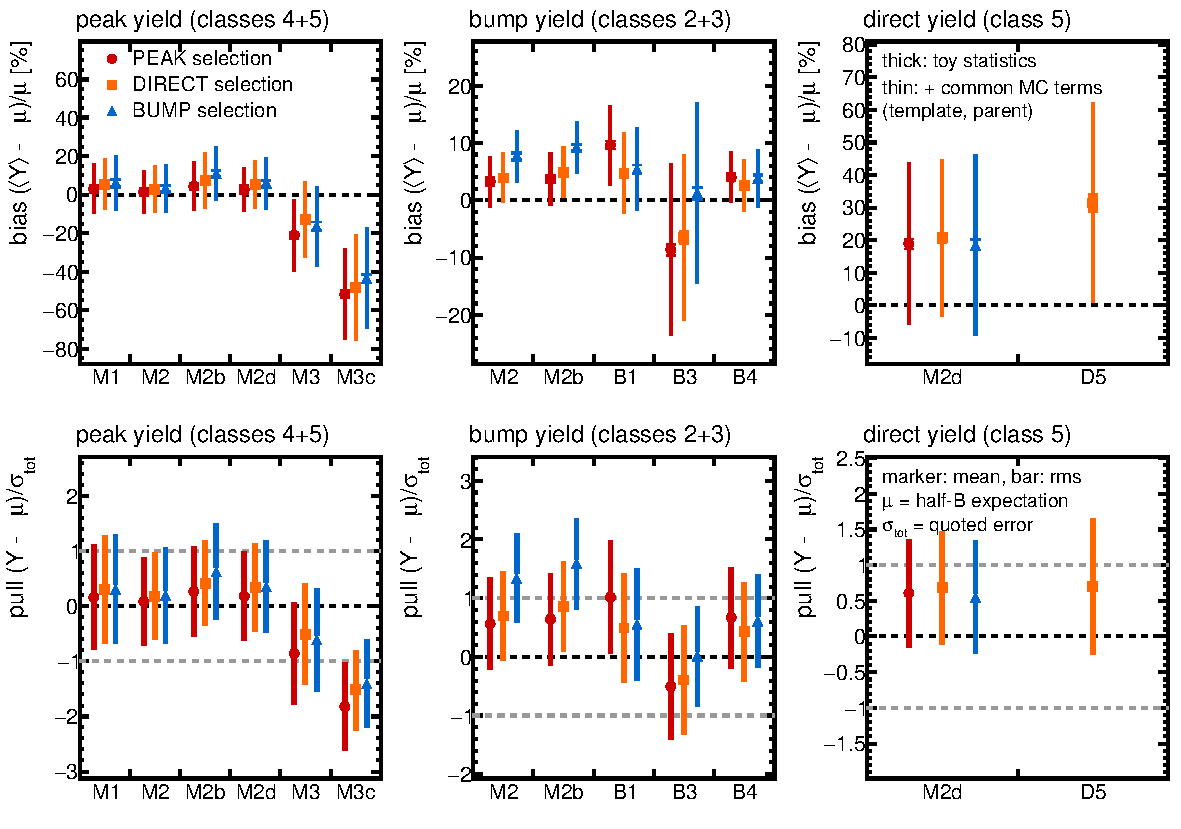
\includegraphics[width=\textwidth]{figs/s5_blind_eval_eta_bias.pdf}
\caption{Blind test, $\eta$ yields. Top: relative bias per method and selection (thick bars: toy statistics,
thin bars: including the common simulation error). Bottom: pull, marker = mean, bar = rms.}
\label{fig:bias}
\end{figure}

\begin{figure}[H]
\centering
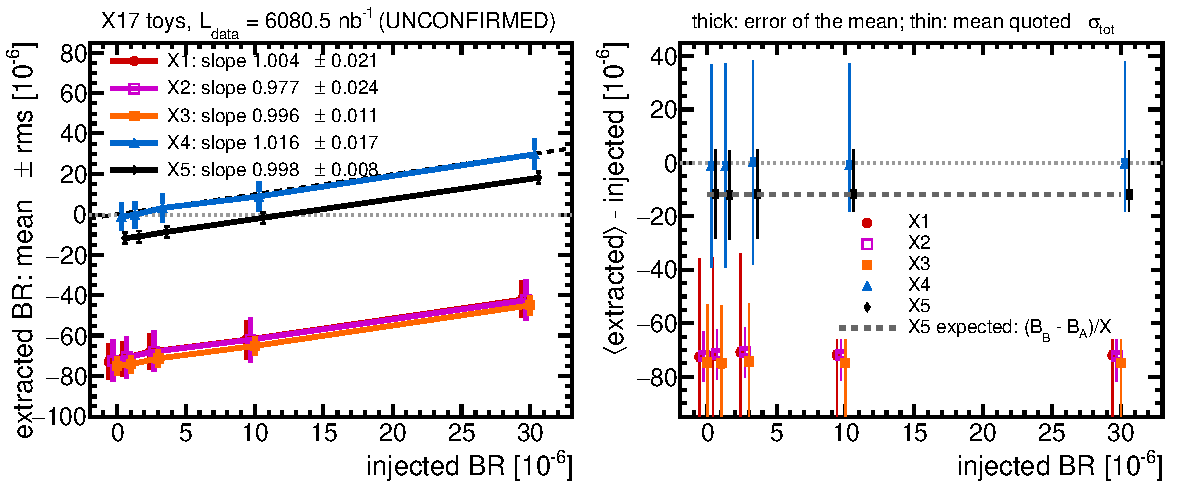
\includegraphics[width=\textwidth]{figs/s5_blind_eval_x17_linearity.pdf}
\caption{Blind test, X17: extracted against injected branching ratio (300 toys per point) with
straight-line fits, and the offset at zero. All estimators follow the injected value with slope 0.98--1.02;
the common offset comes from the background of the simulation sample.}
\label{fig:x17}
\end{figure}

\textbf{What follows.}
\begin{itemize}
\item \textbf{Peak:} the template fit and the calibrated Gaussian fit reproduce the truth within a few per cent;
      in a single data set they may differ from each other by about 12\,\%. Linear side bands lose 20--45\,\%
      because the background is convex under the peak.
\item \textbf{Bump:} the side band with the simulated background shape is closest; the edge step is unbiased
      but imprecise.
\item \textbf{Direct decay alone:} \Mfour cannot separate it from the conversion peak; the split is limited by
      the 307 simulated rows of the conversion channel.
\item \textbf{X17:} the response is linear; a valid limit must include the uncertainty of the background,
      otherwise a background fluctuation can fake a signal (Fig.~\ref{fig:x17}).
\item The quoted errors describe the spread of the toys; the common simulation error must be added.
\end{itemize}

%======================================================================
\section{Open points}
%======================================================================
\begin{itemize}
\item $\Ldata$ to be confirmed; no CB in this study (the cut choice must be repeated with data).
\item The standard set limits the bump, conversion and X17-background templates: a larger production would
      reduce the dominant simulation error.
\item Producers: confirm the HGeant $\eta\to\ee\gamma$ setting (6.0\,\%) and regenerate the $\eta$ set with a
      dilepton definition of $\eta\to\ppee$.
\item Beam energy: the analysis uses $T = 4530$\,MeV, SMASH 4500\,MeV (affects the missing mass only).
\end{itemize}

\end{document}
